\documentclass[compress]{beamer}
\usetheme{sthlm}

%-=-=-=-=-=-=-=-=-=-=-=-=-=-=-=-=-=-=-=-=-=-=-=-=
%        LOADING BEAMER PACKAGES
%-=-=-=-=-=-=-=-=-=-=-=-=-=-=-=-=-=-=-=-=-=-=-=-=

\usepackage{
booktabs,
datetime,
dtk-logos,
graphicx,
multicol,
pgfplots,
ragged2e,
tabularx,
tikz,
wasysym,
multirow,
float,
caption,
subcaption
}

\pgfplotsset{compat=1.8}

\usepackage[utf8]{inputenc}
\usepackage[portuguese]{babel}
\usepackage[T1]{fontenc}
\usepackage{newpxtext,newpxmath}
\usepackage{listings}

\lstset{ %
language=[LaTeX]TeX,
basicstyle=\normalsize\ttfamily,
keywordstyle=,
numbers=left,
numberstyle=\tiny\ttfamily,
stepnumber=1,
showspaces=false,
showstringspaces=false,
showtabs=false,
breaklines=true,
frame=tb,
framerule=0.5pt,
tabsize=4,
framexleftmargin=0.5em,
framexrightmargin=0.5em,
xleftmargin=0.5em,
xrightmargin=0.5em
}



%-=-=-=-=-=-=-=-=-=-=-=-=-=-=-=-=-=-=-=-=-=-=-=-=
%        LOADING TIKZ LIBRARIES
%-=-=-=-=-=-=-=-=-=-=-=-=-=-=-=-=-=-=-=-=-=-=-=-=

\usetikzlibrary{
backgrounds,
mindmap
}

%-=-=-=-=-=-=-=-=-=-=-=-=-=-=-=-=-=-=-=-=-=-=-=-=
%        BEAMER OPTIONS
%-=-=-=-=-=-=-=-=-=-=-=-=-=-=-=-=-=-=-=-=-=-=-=-=

\setbeameroption{show notes}

%-=-=-=-=-=-=-=-=-=-=-=-=-=-=-=-=-=-=-=-=-=-=-=-=
%        BEAMER COMMANDS
%-=-=-=-=-=-=-=-=-=-=-=-=-=-=-=-=-=-=-=-=-=-=-=-=


%-=-=-=-=-=-=-=-=-=-=-=-=-=-=-=-=-=-=-=-=-=-=-=-=
%
%	PRESENTATION INFORMATION
%
%-=-=-=-=-=-=-=-=-=-=-=-=-=-=-=-=-=-=-=-=-=-=-=-=

\title{Modelos persistentes de comunicação por mensagens}
\subtitle{DCE540 - Computação Paralela e Distribuída}
%\date{\small{\jobname}}
\author{\texttt{Iago Carvalho}}
\institute{\texttt{Departamento de Ciência da Computação}}

\hypersetup{
pdfauthor = {Iago A. Carvalho},      
pdfsubject = {Computação Paralela e Distribuída},
pdfkeywords = {},  
pdfmoddate= {D:\pdfdate},          
pdfcreator = {WriteLaTeX}
}

\begin{document}

\begin{frame}
\titlepage

\end{frame}

%% --------------------------------------------------------

\begin{frame}{Mensagens persistentes}

Como vimos nas aulas anteriores, os métodos de comunicação existentes utilizam mensagens transientes

\vspace{0.5cm}

Entretanto, é possível implementar um sistema de mensagens persistentes no \textit{middleware} de um sistema distribuído

\vspace{0.5cm}

Existe um número de diferentes implementações. Entretanto, as mais utilizadas são
\begin{itemize}
    \item Fila de mensagens
    \item \textit{Message broker}
\end{itemize}

\end{frame}

%% --------------------------------------------------------

\begin{frame}{Fila de mensagens}

Componentes não comunicam-se diretamente uns com os outros
\begin{itemize}
    \item Mensagens são depositadas em filas (buffers)
    \item Componente específico para gerenciar as filas
    \item Mensagens são encaminhadas para o destinatário
\end{itemize} 

\vspace{0.5cm}

Cada componente possui sua própria fila
\begin{itemize}
    \item Outros componentes podem enviar mensagens, mas não tem acesso de leitura
\end{itemize}

\vspace{0.5cm}

É possível criar filas compartilhadas por diversos componentes
\begin{itemize}
    \item Uma maneira interessante de obtermos computação paralela
    \item Balancemaneto de carga
\end{itemize}

\end{frame}

%% --------------------------------------------------------

\begin{frame}{Fila de mensagens - Computação paralela}

\vspace{0.5cm}

\centering 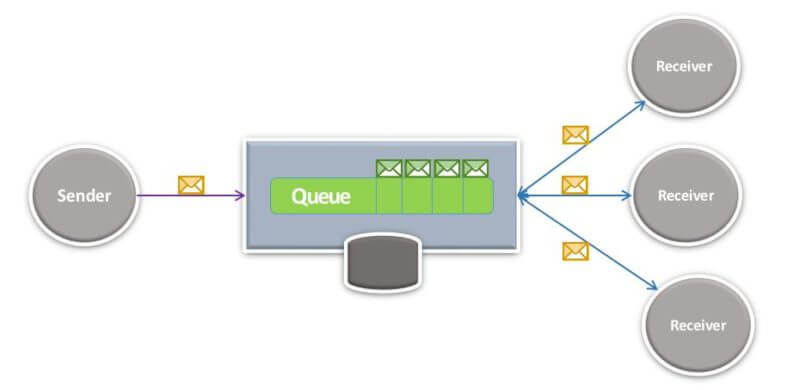
\includegraphics[width=\textwidth]{images/queue_paralela.png}

\end{frame}

%% --------------------------------------------------------

\begin{frame}{Fila de mensagens}

Este sistema permite que tenhamos comunicação persistente

\vspace{0.75cm}

\centering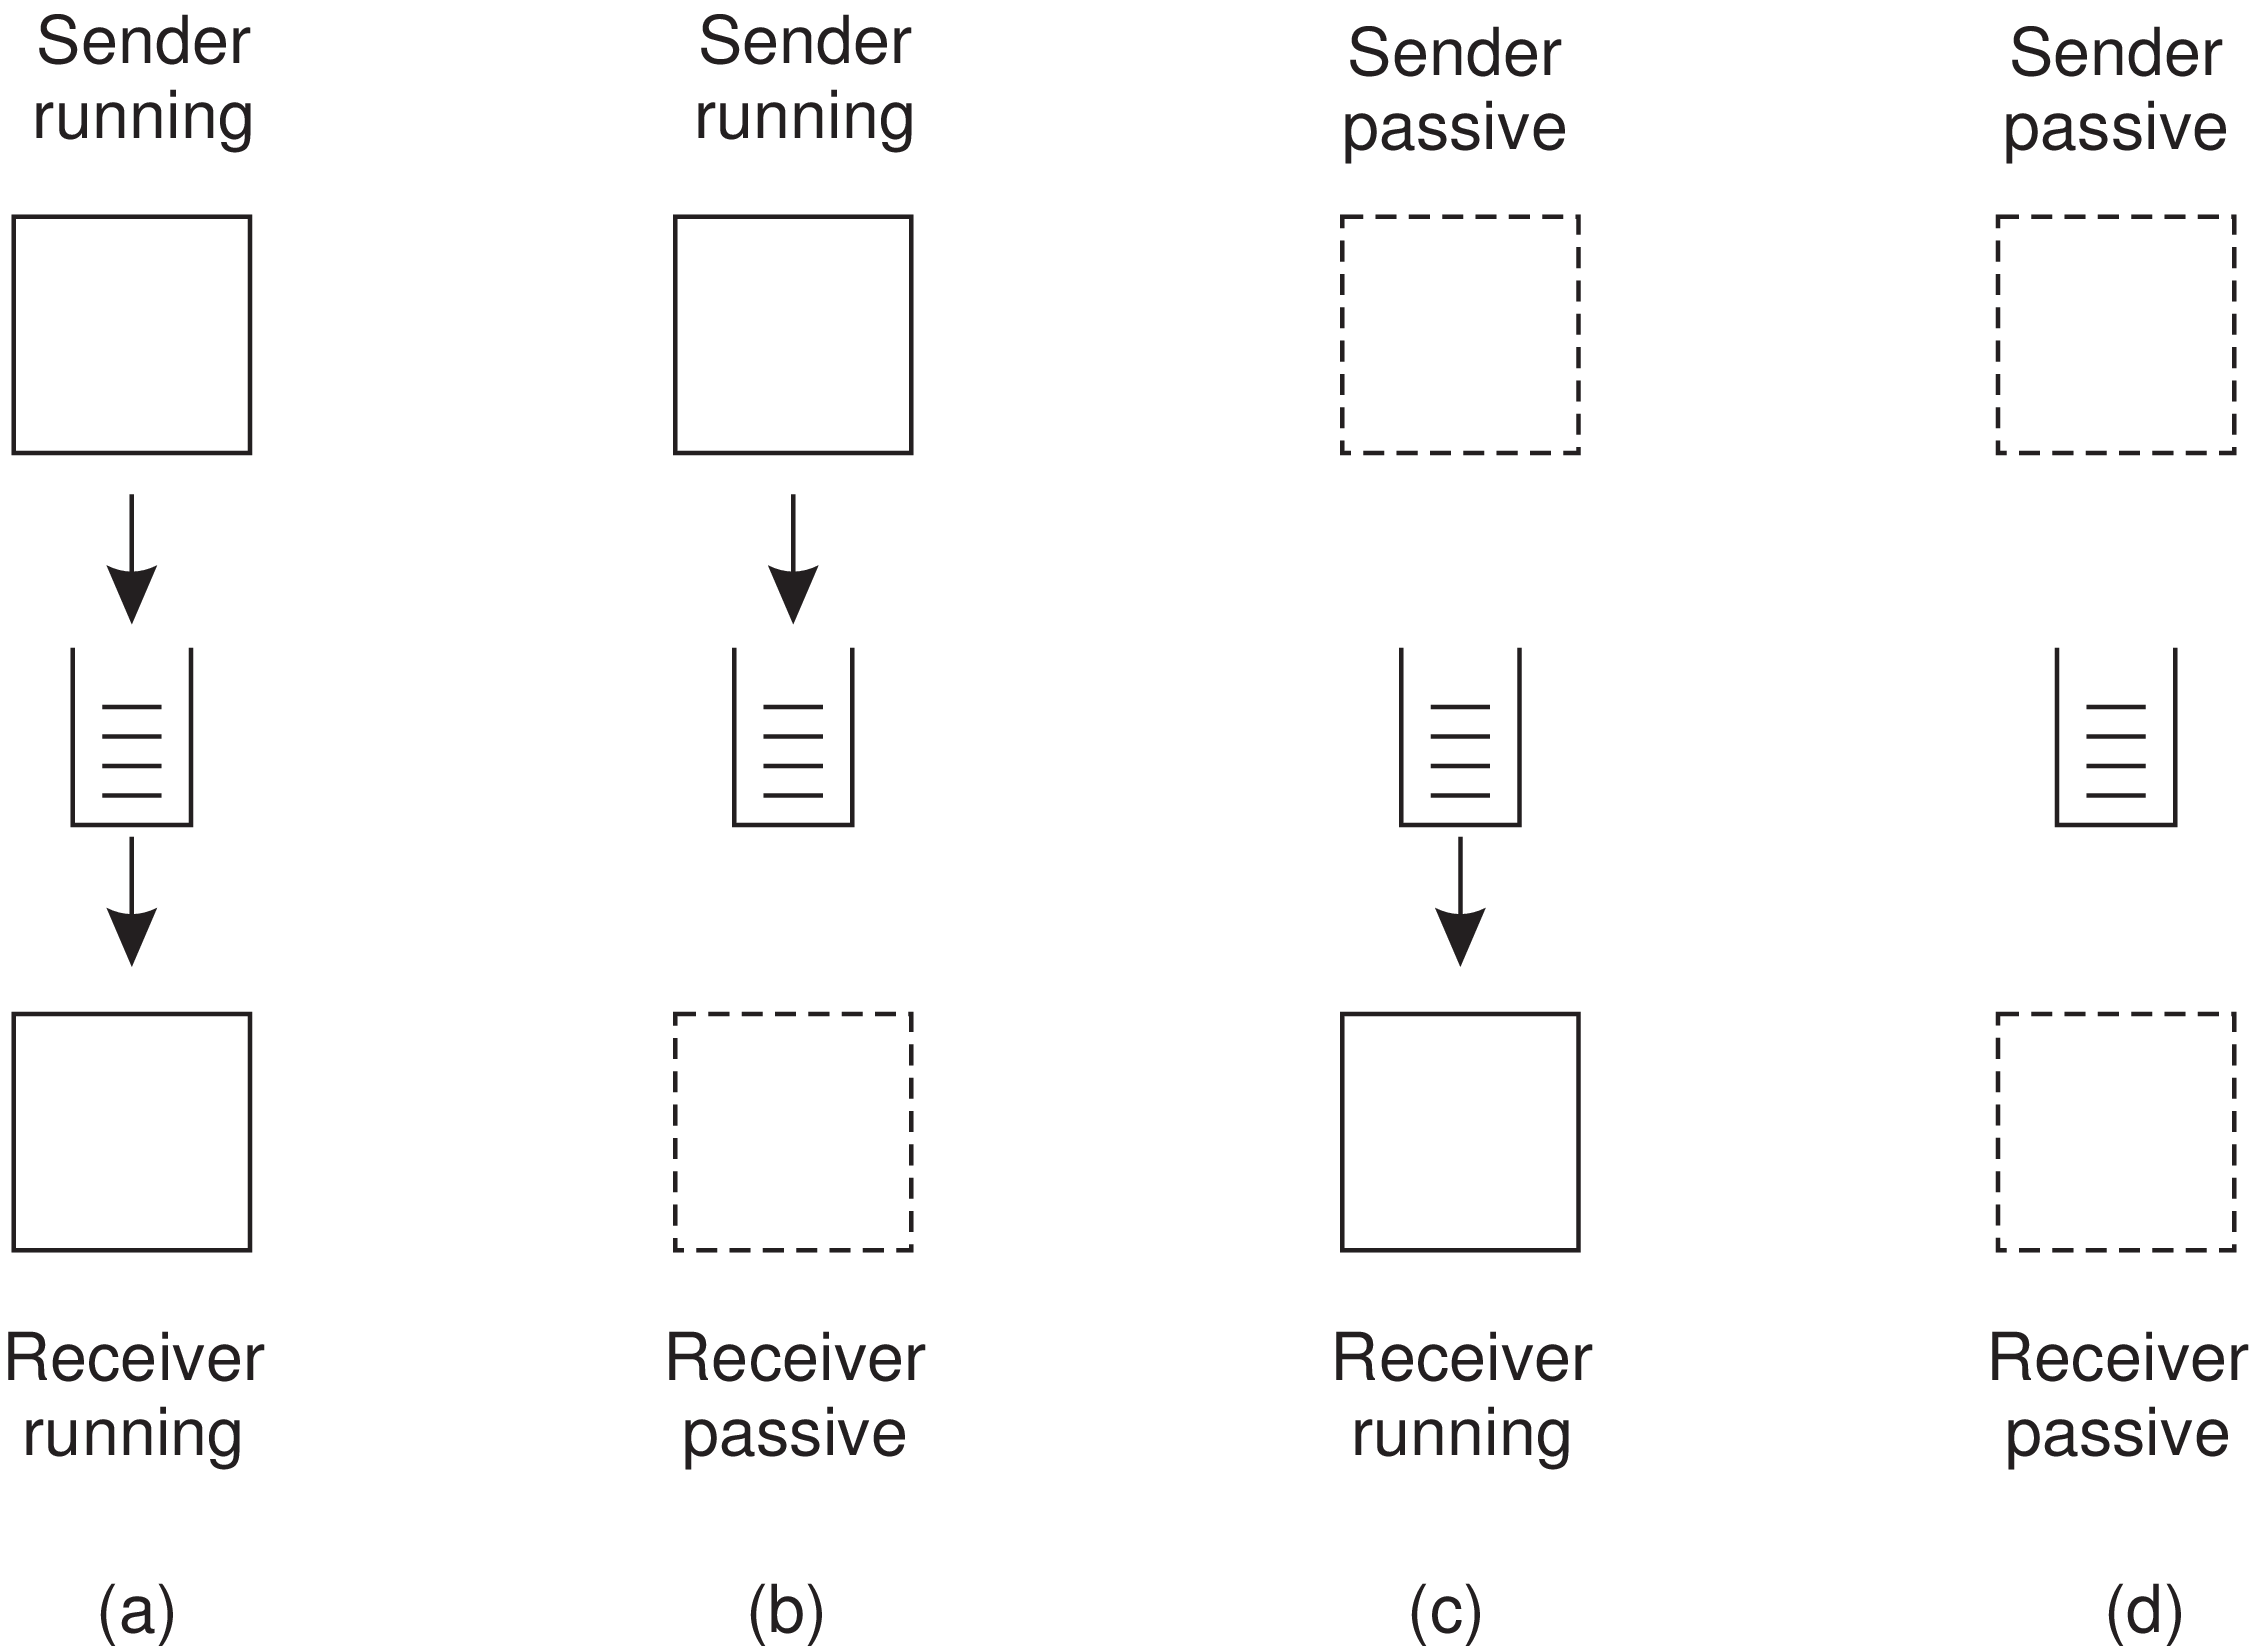
\includegraphics[width=0.9\textwidth]{images/transmissao_filas.png}

\end{frame}

%% --------------------------------------------------------

\begin{frame}{\textit{Middleware} e fila de mensagens}

\textit{Middleware} deve fornecer quatro operações básicas em uma fila de mensagens

\begin{enumerate}
    \item put \textcolor{sthlmDarkBlue}{$\leftarrow$} adiciona uma mensagem a uma fila
    \item get \textcolor{sthlmDarkBlue}{$\leftarrow$} obtem uma mensagem da fila; processo bloqueado até que fila não-vazia
    \item poll \textcolor{sthlmDarkBlue}{$\leftarrow$} checa se existe mensagem em uma fila. Em caso positivo, obtem a mensagem
    \item notify \textcolor{sthlmDarkBlue}{$\leftarrow$} pede para receber uma notificação quando uma mensagem chegar
\end{enumerate}

\vspace{0.5cm}

Um \textit{middleware} consegue garantir ao remetente que a mensagem será postada
\begin{itemize}
    \item Entretanto, é impossível garantir que a mensagem será lida
    \item Operação adicional: notificação de mensagem lida
\end{itemize}
\end{frame}

%% --------------------------------------------------------

\begin{frame}{\textit{Message broker}}

Filas de mensagens são excelentes maneiras para fazer a troca de mensagens de forma persistente em sistemas distribuídos
\begin{itemize}
    \item Sistemas bem controlados
\end{itemize}

\vspace{0.25cm}

Entretanto, em sistemas distribuídos mais dinâmicos (com uma frequente inserção e remoção de componentes), usar uma fila de mensagens pode não ser uma boa ideia
\begin{itemize}
    \item Cada componente pode usar seu próprio protocolo para troca de mensagens
    \item Mensagens precisam ser convertidas entre cada componente
\end{itemize}

\vspace{0.25cm}

Soluções possíveis
\begin{itemize}
    \item Implementar $N^2$ interfaces para tradução de mensagens
    \begin{itemize}
        \item Implementar $N$ novas interfaces para cada componente
    \end{itemize}
    \item Componente dedicado para a tradução de mensagens
\end{itemize}
\end{frame}

%% --------------------------------------------------------

\begin{frame}{\textit{Message broker}}

Um \textit{message broker} atua como um \textit{gateway} em uma fila de mensagens

\vspace{0.5cm}

\centering 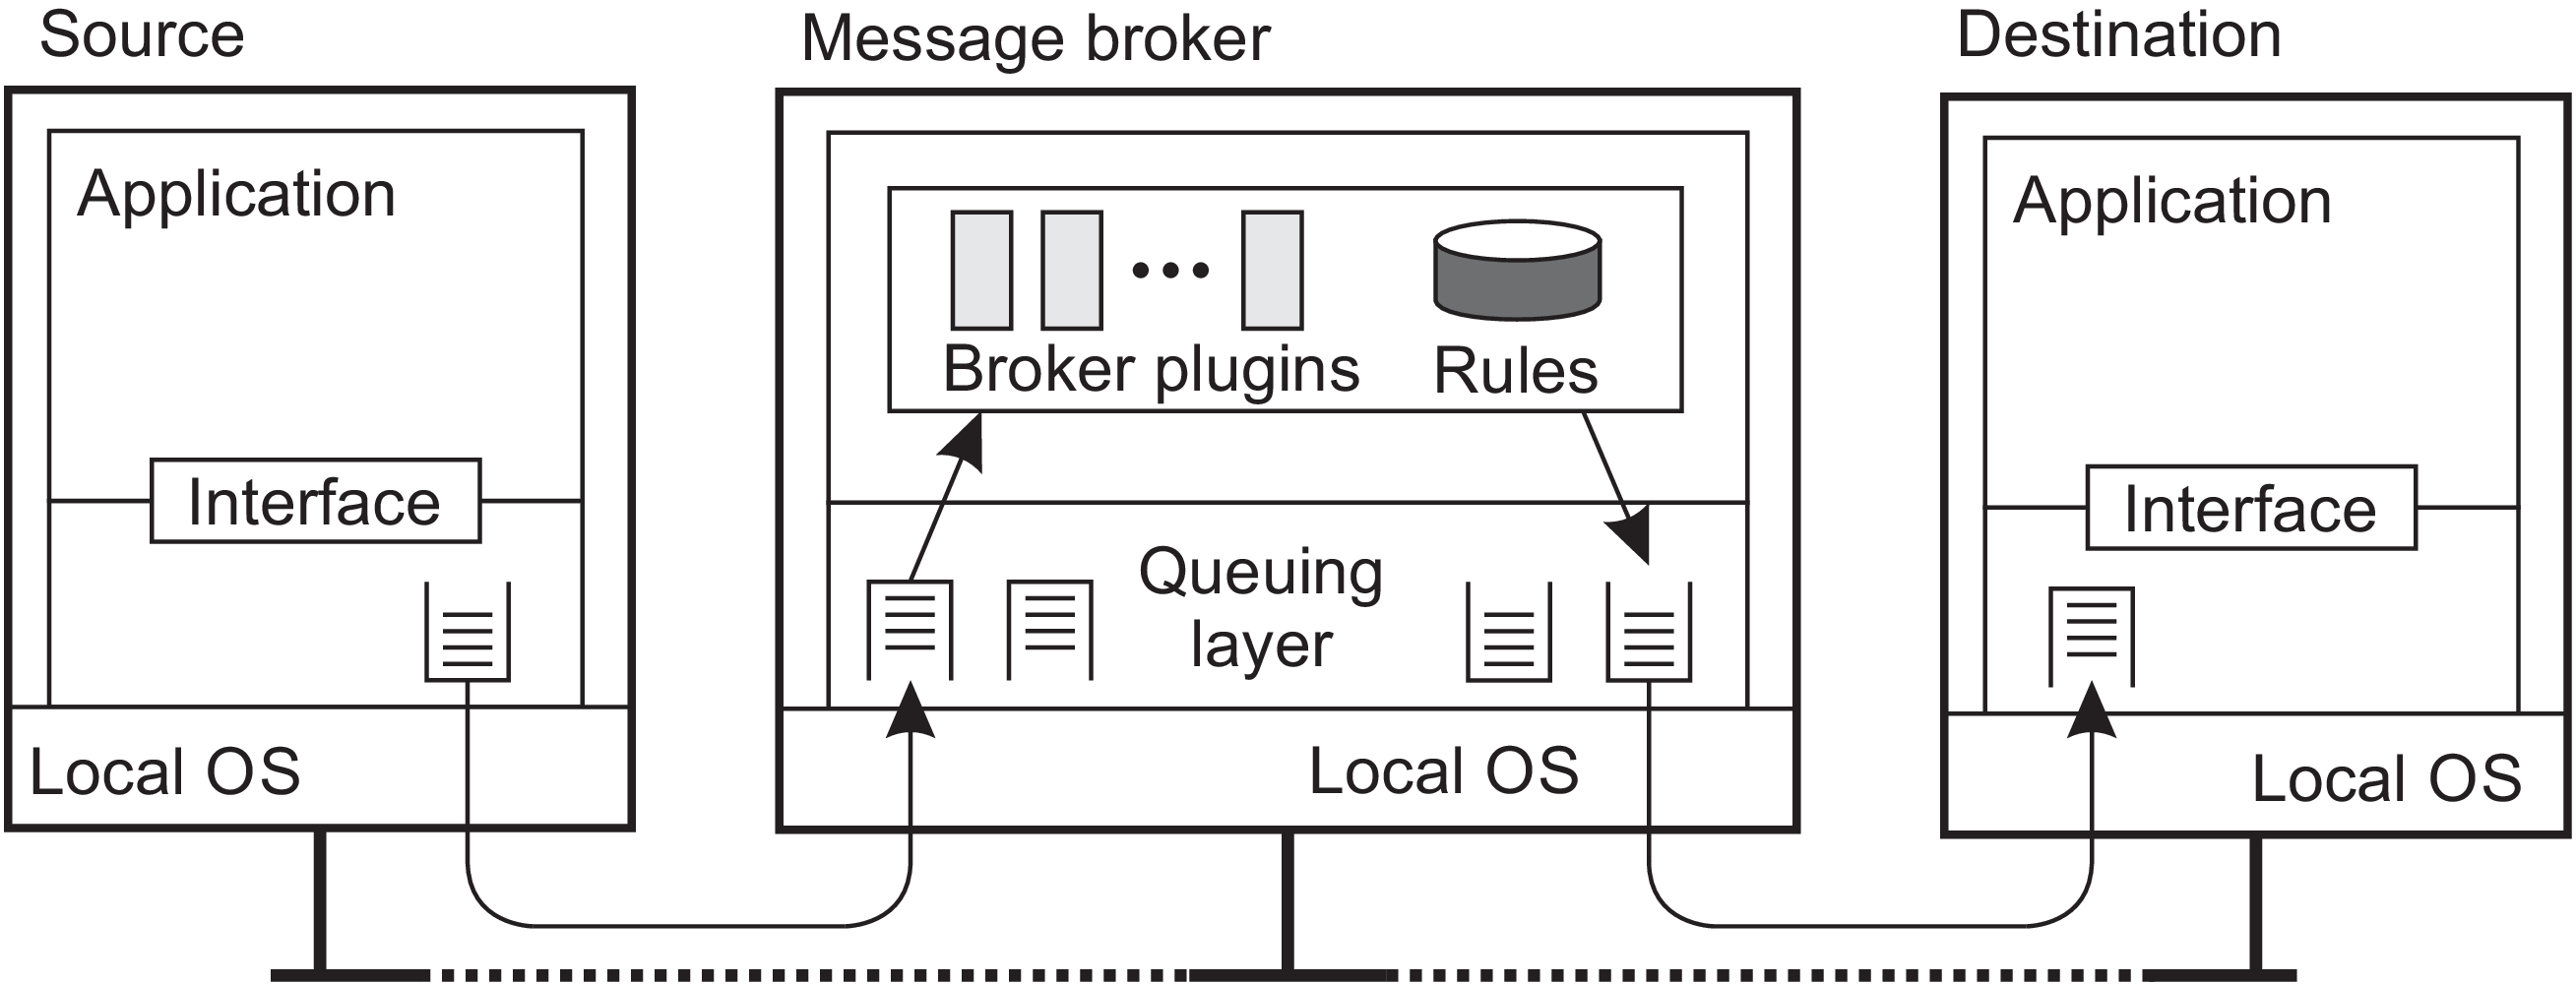
\includegraphics[width=\textwidth]{images/broker.png}
\end{frame}

\end{document}
